\documentclass[1p]{elsarticle_modified}
%\bibliographystyle{elsarticle-num}

%\usepackage[colorlinks]{hyperref}
%\usepackage{abbrmath_seonhwa} %\Abb, \Ascr, \Acal ,\Abf, \Afrak
\usepackage{amsfonts}
\usepackage{amssymb}
\usepackage{amsmath}
\usepackage{amsthm}
\usepackage{scalefnt}
\usepackage{amsbsy}
\usepackage{kotex}
\usepackage{caption}
\usepackage{subfig}
\usepackage{color}
\usepackage{graphicx}
\usepackage{xcolor} %% white, black, red, green, blue, cyan, magenta, yellow
\usepackage{float}
\usepackage{setspace}
\usepackage{hyperref}

\usepackage{tikz}
\usetikzlibrary{arrows}

\usepackage{multirow}
\usepackage{array} % fixed length table
\usepackage{hhline}

%%%%%%%%%%%%%%%%%%%%%
\makeatletter
\renewcommand*\env@matrix[1][\arraystretch]{%
	\edef\arraystretch{#1}%
	\hskip -\arraycolsep
	\let\@ifnextchar\new@ifnextchar
	\array{*\c@MaxMatrixCols c}}
\makeatother %https://tex.stackexchange.com/questions/14071/how-can-i-increase-the-line-spacing-in-a-matrix
%%%%%%%%%%%%%%%

\usepackage[normalem]{ulem}

\newcommand{\msout}[1]{\ifmmode\text{\sout{\ensuremath{#1}}}\else\sout{#1}\fi}
%SOURCE: \msout is \stkout macro in https://tex.stackexchange.com/questions/20609/strikeout-in-math-mode

\newcommand{\cancel}[1]{
	\ifmmode
	{\color{red}\msout{#1}}
	\else
	{\color{red}\sout{#1}}
	\fi
}

\newcommand{\add}[1]{
	{\color{blue}\uwave{#1}}
}

\newcommand{\replace}[2]{
	\ifmmode
	{\color{red}\msout{#1}}{\color{blue}\uwave{#2}}
	\else
	{\color{red}\sout{#1}}{\color{blue}\uwave{#2}}
	\fi
}

\newcommand{\Sol}{\mathcal{S}} %segment
\newcommand{\D}{D} %diagram
\newcommand{\A}{\mathcal{A}} %arc


%%%%%%%%%%%%%%%%%%%%%%%%%%%%%5 test

\def\sl{\operatorname{\textup{SL}}(2,\Cbb)}
\def\psl{\operatorname{\textup{PSL}}(2,\Cbb)}
\def\quan{\mkern 1mu \triangleright \mkern 1mu}

\theoremstyle{definition}
\newtheorem{thm}{Theorem}[section]
\newtheorem{prop}[thm]{Proposition}
\newtheorem{lem}[thm]{Lemma}
\newtheorem{ques}[thm]{Question}
\newtheorem{cor}[thm]{Corollary}
\newtheorem{defn}[thm]{Definition}
\newtheorem{exam}[thm]{Example}
\newtheorem{rmk}[thm]{Remark}
\newtheorem{alg}[thm]{Algorithm}

\newcommand{\I}{\sqrt{-1}}
\begin{document}

%\begin{frontmatter}
%
%\title{Boundary parabolic representations of knots up to 8 crossings}
%
%%% Group authors per affiliation:
%\author{Yunhi Cho} 
%\address{Department of Mathematics, University of Seoul, Seoul, Korea}
%\ead{yhcho@uos.ac.kr}
%
%
%\author{Seonhwa Kim} %\fnref{s_kim}}
%\address{Center for Geometry and Physics, Institute for Basic Science, Pohang, 37673, Korea}
%\ead{ryeona17@ibs.re.kr}
%
%\author{Hyuk Kim}
%\address{Department of Mathematical Sciences, Seoul National University, Seoul 08826, Korea}
%\ead{hyukkim@snu.ac.kr}
%
%\author{Seokbeom Yoon}
%\address{Department of Mathematical Sciences, Seoul National University, Seoul, 08826,  Korea}
%\ead{sbyoon15@snu.ac.kr}
%
%\begin{abstract}
%We find all boundary parabolic representation of knots up to 8 crossings.
%
%\end{abstract}
%\begin{keyword}
%    \MSC[2010] 57M25 
%\end{keyword}
%
%\end{frontmatter}

%\linenumbers
%\tableofcontents
%
\newcommand\colored[1]{\textcolor{white}{\rule[-0.35ex]{0.8em}{1.4ex}}\kern-0.8em\color{red} #1}%
%\newcommand\colored[1]{\textcolor{white}{ #1}\kern-2.17ex	\textcolor{white}{ #1}\kern-1.81ex	\textcolor{white}{ #1}\kern-2.15ex\color{red}#1	}

{\Large $\underline{11n_{173}~(K11n_{173})}$}

\setlength{\tabcolsep}{10pt}
\renewcommand{\arraystretch}{1.6}
\vspace{1cm}\begin{tabular}{m{100pt}>{\centering\arraybackslash}m{274pt}}
\multirow{5}{120pt}{
	\centering
	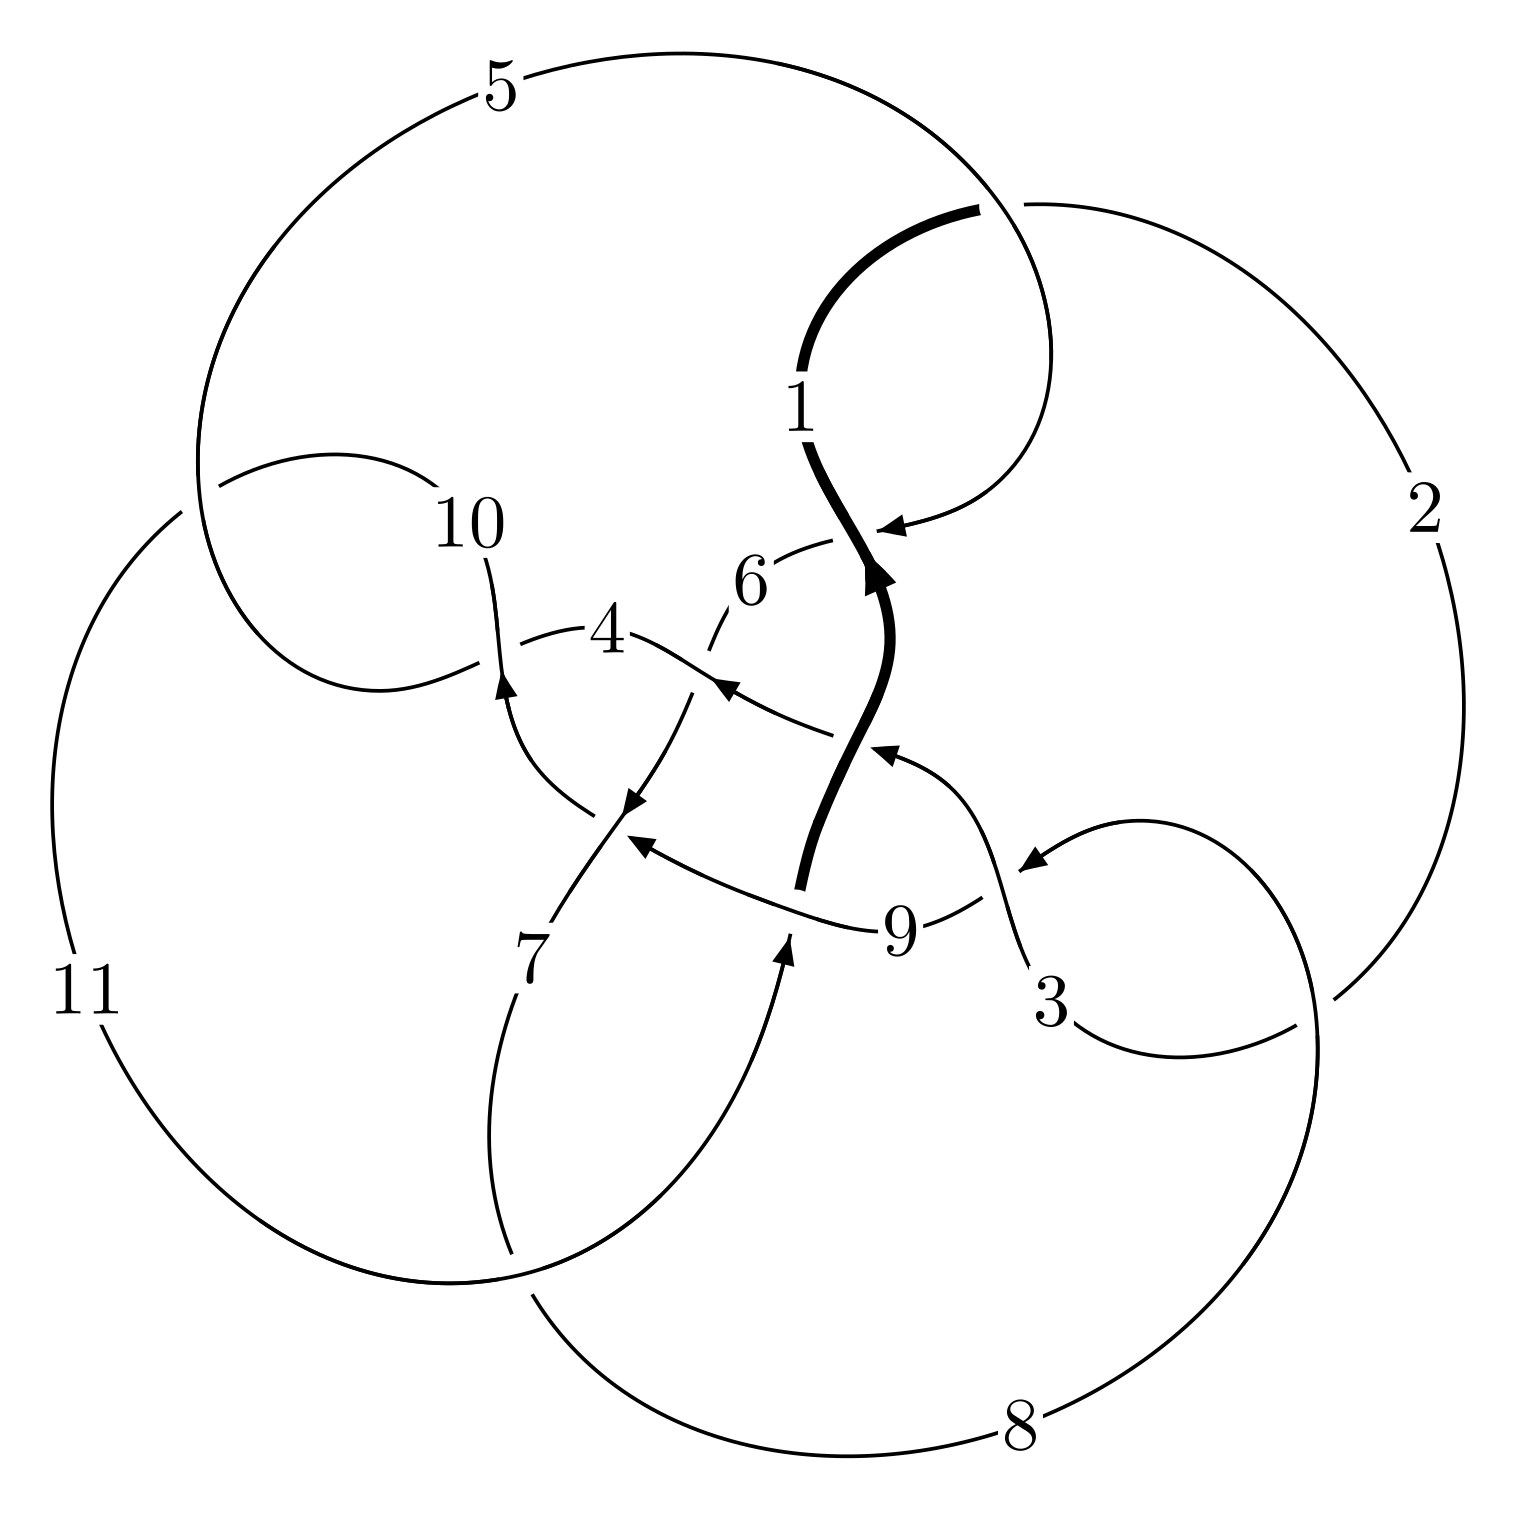
\includegraphics[width=112pt]{../../../GIT/diagram.site/Diagrams/png/789_11n_173.png}\\
\ \ \ A knot diagram\footnotemark}&
\allowdisplaybreaks
\textbf{Linearized knot diagam} \\
\cline{2-2}
 &
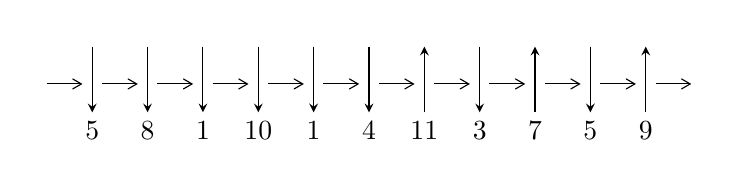
\begin{tikzpicture}[x=20pt, y=17pt]
	% nodes
	\node (C0) at (0, 0) {};
	\node (C1) at (1, 0) {};
	\node (C1U) at (1, +1) {};
	\node (C1D) at (1, -1) {5};

	\node (C2) at (2, 0) {};
	\node (C2U) at (2, +1) {};
	\node (C2D) at (2, -1) {8};

	\node (C3) at (3, 0) {};
	\node (C3U) at (3, +1) {};
	\node (C3D) at (3, -1) {1};

	\node (C4) at (4, 0) {};
	\node (C4U) at (4, +1) {};
	\node (C4D) at (4, -1) {10};

	\node (C5) at (5, 0) {};
	\node (C5U) at (5, +1) {};
	\node (C5D) at (5, -1) {1};

	\node (C6) at (6, 0) {};
	\node (C6U) at (6, +1) {};
	\node (C6D) at (6, -1) {4};

	\node (C7) at (7, 0) {};
	\node (C7U) at (7, +1) {};
	\node (C7D) at (7, -1) {11};

	\node (C8) at (8, 0) {};
	\node (C8U) at (8, +1) {};
	\node (C8D) at (8, -1) {3};

	\node (C9) at (9, 0) {};
	\node (C9U) at (9, +1) {};
	\node (C9D) at (9, -1) {7};

	\node (C10) at (10, 0) {};
	\node (C10U) at (10, +1) {};
	\node (C10D) at (10, -1) {5};

	\node (C11) at (11, 0) {};
	\node (C11U) at (11, +1) {};
	\node (C11D) at (11, -1) {9};
	\node (C12) at (12, 0) {};

	% arrows
	\draw[->,>={angle 60}]
	(C0) edge (C1) (C1) edge (C2) (C2) edge (C3) (C3) edge (C4) (C4) edge (C5) (C5) edge (C6) (C6) edge (C7) (C7) edge (C8) (C8) edge (C9) (C9) edge (C10) (C10) edge (C11) (C11) edge (C12) ;	\draw[->,>=stealth]
	(C1U) edge (C1D) (C2U) edge (C2D) (C3U) edge (C3D) (C4U) edge (C4D) (C5U) edge (C5D) (C6U) edge (C6D) (C7D) edge (C7U) (C8U) edge (C8D) (C9D) edge (C9U) (C10U) edge (C10D) (C11D) edge (C11U) ;
	\end{tikzpicture} \\
\hhline{~~} \\& 
\textbf{Solving Sequence} \\ \cline{2-2} 
 &
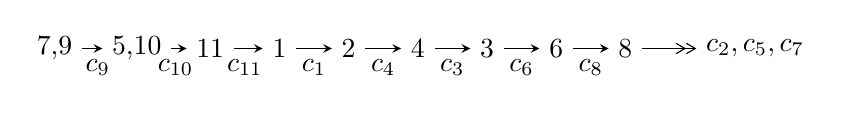
\begin{tikzpicture}[x=25pt, y=7pt]
	% node
	\node (A0) at (-1/8, 0) {7,9};
	\node (A1) at (17/16, 0) {5,10};
	\node (A2) at (17/8, 0) {11};
	\node (A3) at (25/8, 0) {1};
	\node (A4) at (33/8, 0) {2};
	\node (A5) at (41/8, 0) {4};
	\node (A6) at (49/8, 0) {3};
	\node (A7) at (57/8, 0) {6};
	\node (A8) at (65/8, 0) {8};
	\node (C1) at (1/2, -1) {$c_{9}$};
	\node (C2) at (13/8, -1) {$c_{10}$};
	\node (C3) at (21/8, -1) {$c_{11}$};
	\node (C4) at (29/8, -1) {$c_{1}$};
	\node (C5) at (37/8, -1) {$c_{4}$};
	\node (C6) at (45/8, -1) {$c_{3}$};
	\node (C7) at (53/8, -1) {$c_{6}$};
	\node (C8) at (61/8, -1) {$c_{8}$};
	\node (A9) at (10, 0) {$c_{2},c_{5},c_{7}$};

	% edge
	\draw[->,>=stealth]	
	(A0) edge (A1) (A1) edge (A2) (A2) edge (A3) (A3) edge (A4) (A4) edge (A5) (A5) edge (A6) (A6) edge (A7) (A7) edge (A8) ;
	\draw[->>,>={angle 60}]	
	(A8) edge (A9);
\end{tikzpicture} \\ 

\end{tabular} \\

\footnotetext{
The image of knot diagram is generated by the software ``\textbf{Draw programme}" developed by Andrew Bartholomew(\url{http://www.layer8.co.uk/maths/draw/index.htm\#Running-draw}), where we modified some parts for our purpose(\url{https://github.com/CATsTAILs/LinksPainter}).
}\phantom \\ \newline 
\centering \textbf{Ideals for irreducible components\footnotemark of $X_{\text{par}}$} 
 
\begin{align*}
I^u_{1}&=\langle 
616 u^{12}+178 u^{11}+\cdots+1367 b+80,\;654 u^{12}-388 u^{11}+\cdots+1367 a+1807,\\
\phantom{I^u_{1}}&\phantom{= \langle  }u^{13}+3 u^{11}-5 u^{10}+10 u^9-14 u^8+22 u^7-29 u^6+36 u^5-32 u^4+24 u^3-11 u^2+4 u+1\rangle \\
I^u_{2}&=\langle 
- u^4+u^2+b-1,\;a+u-1,\;u^5- u^3- u^2+u+1\rangle \\
I^u_{3}&=\langle 
-7.93323\times10^{30} u^{27}-2.30191\times10^{31} u^{26}+\cdots+1.77551\times10^{32} b-1.02298\times10^{33},\\
\phantom{I^u_{3}}&\phantom{= \langle  }5.27149\times10^{33} u^{27}+4.23845\times10^{33} u^{26}+\cdots+4.70510\times10^{34} a-4.74518\times10^{34},\;u^{28}+2 u^{27}+\cdots+16 u+53\rangle \\
I^u_{4}&=\langle 
-89 u^{13}+200 u^{12}+\cdots+113 b-381,\;134 u^{13}-503 u^{12}+\cdots+113 a-178,\\
\phantom{I^u_{4}}&\phantom{= \langle  }u^{14}-3 u^{13}+4 u^{12}-4 u^{11}- u^{10}+2 u^9-2 u^8+u^7+13 u^6-7 u^5+22 u^4- u^3+8 u^2+1\rangle \\
\\
\end{align*}
\raggedright * 4 irreducible components of $\dim_{\mathbb{C}}=0$, with total 60 representations.\\
\footnotetext{All coefficients of polynomials are rational numbers. But the coefficients are sometimes approximated in decimal forms when there is not enough margin.}
\newpage
\renewcommand{\arraystretch}{1}
\centering \section*{I. $I^u_{1}= \langle 616 u^{12}+178 u^{11}+\cdots+1367 b+80,\;654 u^{12}-388 u^{11}+\cdots+1367 a+1807,\;u^{13}+3 u^{11}+\cdots+4 u+1 \rangle$}
\flushleft \textbf{(i) Arc colorings}\\
\begin{tabular}{m{7pt} m{180pt} m{7pt} m{180pt} }
\flushright $a_{7}=$&$\begin{pmatrix}0\\u\end{pmatrix}$ \\
\flushright $a_{9}=$&$\begin{pmatrix}1\\0\end{pmatrix}$ \\
\flushright $a_{5}=$&$\begin{pmatrix}-0.478420 u^{12}+0.283833 u^{11}+\cdots+4.18288 u-1.32187\\-0.450622 u^{12}-0.130212 u^{11}+\cdots+1.21507 u-0.0585223\end{pmatrix}$ \\
\flushright $a_{10}=$&$\begin{pmatrix}1\\- u^2\end{pmatrix}$ \\
\flushright $a_{11}=$&$\begin{pmatrix}-0.384784 u^{12}-0.637162 u^{11}+\cdots-4.49817 u+1.19678\\- u\end{pmatrix}$ \\
\flushright $a_{1}=$&$\begin{pmatrix}-0.384784 u^{12}-0.637162 u^{11}+\cdots-5.49817 u+1.19678\\- u\end{pmatrix}$ \\
\flushright $a_{2}=$&$\begin{pmatrix}-0.513533 u^{12}-1.24579 u^{11}+\cdots-9.43672 u+1.60863\\0.319678 u^{12}+0.238478 u^{11}+\cdots-1.62985 u+0.0285296\end{pmatrix}$ \\
\flushright $a_{4}=$&$\begin{pmatrix}-0.314557 u^{12}+0.422092 u^{11}+\cdots+4.74104 u-1.66423\\-0.286028 u^{12}+0.102414 u^{11}+\cdots+1.93197 u+0.0797366\end{pmatrix}$ \\
\flushright $a_{3}=$&$\begin{pmatrix}-0.228237 u^{12}-0.442575 u^{11}+\cdots+2.47257 u-2.95172\\0.163862 u^{12}+0.138259 u^{11}+\cdots+0.558157 u-0.342356\end{pmatrix}$ \\
\flushright $a_{6}=$&$\begin{pmatrix}-1.17776 u^{12}-0.931236 u^{11}+\cdots+0.425750 u-0.789320\\-0.514996 u^{12}-0.434528 u^{11}+\cdots-0.754206 u-0.352597\end{pmatrix}$ \\
\flushright $a_{8}=$&$\begin{pmatrix}-0.259693 u^{12}-1.50037 u^{11}+\cdots-5.35333 u-1.61814\\0.193855 u^{12}+0.00731529 u^{11}+\cdots-1.93343 u-0.637162\end{pmatrix}$\\ \flushright $a_{8}=$&$\begin{pmatrix}-0.259693 u^{12}-1.50037 u^{11}+\cdots-5.35333 u-1.61814\\0.193855 u^{12}+0.00731529 u^{11}+\cdots-1.93343 u-0.637162\end{pmatrix}$\\&\end{tabular}
\flushleft \textbf{(ii) Obstruction class $= -1$}\\~\\
\flushleft \textbf{(iii) Cusp Shapes $= -\frac{2267}{1367} u^{12}-\frac{1272}{1367} u^{11}-\frac{8216}{1367} u^{10}+\frac{5428}{1367} u^9-\frac{22362}{1367} u^8+\frac{19107}{1367} u^7-\frac{40203}{1367} u^6+\frac{45449}{1367} u^5-\frac{57148}{1367} u^4+\frac{42609}{1367} u^3-\frac{31315}{1367} u^2+\frac{5649}{1367} u-\frac{15793}{1367}$}\\~\\
\newpage\renewcommand{\arraystretch}{1}
\flushleft \textbf{(iv) u-Polynomials at the component}\newline \\
\begin{tabular}{m{50pt}|m{274pt}}
Crossings & \hspace{64pt}u-Polynomials at each crossing \\
\hline $$\begin{aligned}c_{1},c_{5}\end{aligned}$$&$\begin{aligned}
&u^{13}+8 u^{12}+\cdots-10 u+4
\end{aligned}$\\
\hline $$\begin{aligned}c_{2},c_{4},c_{8}\\c_{10}\end{aligned}$$&$\begin{aligned}
&u^{13}-8 u^{11}+\cdots-2 u+2
\end{aligned}$\\
\hline $$\begin{aligned}c_{3},c_{6}\end{aligned}$$&$\begin{aligned}
&u^{13}-2 u^{12}+\cdots-3 u+1
\end{aligned}$\\
\hline $$\begin{aligned}c_{7}\end{aligned}$$&$\begin{aligned}
&u^{13}-10 u^{12}+\cdots-40 u+20
\end{aligned}$\\
\hline $$\begin{aligned}c_{9},c_{11}\end{aligned}$$&$\begin{aligned}
&u^{13}+3 u^{11}+\cdots+4 u+1
\end{aligned}$\\
\hline
\end{tabular}\\~\\
\newpage\renewcommand{\arraystretch}{1}
\flushleft \textbf{(v) Riley Polynomials at the component}\newline \\
\begin{tabular}{m{50pt}|m{274pt}}
Crossings & \hspace{64pt}Riley Polynomials at each crossing \\
\hline $$\begin{aligned}c_{1},c_{5}\end{aligned}$$&$\begin{aligned}
&y^{13}-16 y^{12}+\cdots+284 y-16
\end{aligned}$\\
\hline $$\begin{aligned}c_{2},c_{4},c_{8}\\c_{10}\end{aligned}$$&$\begin{aligned}
&y^{13}-16 y^{12}+\cdots+12 y-4
\end{aligned}$\\
\hline $$\begin{aligned}c_{3},c_{6}\end{aligned}$$&$\begin{aligned}
&y^{13}-24 y^{12}+\cdots-7 y-1
\end{aligned}$\\
\hline $$\begin{aligned}c_{7}\end{aligned}$$&$\begin{aligned}
&y^{13}-2 y^{12}+\cdots+4440 y-400
\end{aligned}$\\
\hline $$\begin{aligned}c_{9},c_{11}\end{aligned}$$&$\begin{aligned}
&y^{13}+6 y^{12}+\cdots+38 y-1
\end{aligned}$\\
\hline
\end{tabular}\\~\\
\newpage\flushleft \textbf{(vi) Complex Volumes and Cusp Shapes}
$$\begin{array}{c|c|c}  
\text{Solutions to }I^u_{1}& \I (\text{vol} + \sqrt{-1}CS) & \text{Cusp shape}\\
 \hline 
\begin{aligned}
u &= \phantom{-}0.949645 + 0.417400 I \\
a &= -0.333458 - 0.234834 I \\
b &= \phantom{-}0.346830 + 0.825972 I\end{aligned}
 & \phantom{-}1.81165 + 1.04217 I & \phantom{-}4.67201 - 2.86908 I \\ \hline\begin{aligned}
u &= \phantom{-}0.949645 - 0.417400 I \\
a &= -0.333458 + 0.234834 I \\
b &= \phantom{-}0.346830 - 0.825972 I\end{aligned}
 & \phantom{-}1.81165 - 1.04217 I & \phantom{-}4.67201 + 2.86908 I \\ \hline\begin{aligned}
u &= \phantom{-}0.654297 + 0.696942 I \\
a &= \phantom{-}0.22522 + 2.10852 I \\
b &= \phantom{-}0.476213 - 0.178047 I\end{aligned}
 & -13.48820 + 1.07762 I & -12.25276 - 5.21840 I \\ \hline\begin{aligned}
u &= \phantom{-}0.654297 - 0.696942 I \\
a &= \phantom{-}0.22522 - 2.10852 I \\
b &= \phantom{-}0.476213 + 0.178047 I\end{aligned}
 & -13.48820 - 1.07762 I & -12.25276 + 5.21840 I \\ \hline\begin{aligned}
u &= \phantom{-}0.326551 + 0.994649 I \\
a &= \phantom{-}0.241683 - 0.736746 I \\
b &= -0.03079 - 1.57197 I\end{aligned}
 & -4.25079 + 1.54146 I & -6.85137 - 4.44536 I \\ \hline\begin{aligned}
u &= \phantom{-}0.326551 - 0.994649 I \\
a &= \phantom{-}0.241683 + 0.736746 I \\
b &= -0.03079 + 1.57197 I\end{aligned}
 & -4.25079 - 1.54146 I & -6.85137 + 4.44536 I \\ \hline\begin{aligned}
u &= -0.003594 + 0.899426 I \\
a &= -1.89385 - 0.60583 I \\
b &= -0.370370 - 0.914227 I\end{aligned}
 & -5.78882 + 3.81724 I & -10.21345 - 4.30874 I \\ \hline\begin{aligned}
u &= -0.003594 - 0.899426 I \\
a &= -1.89385 + 0.60583 I \\
b &= -0.370370 + 0.914227 I\end{aligned}
 & -5.78882 - 3.81724 I & -10.21345 + 4.30874 I \\ \hline\begin{aligned}
u &= -0.80574 + 1.33514 I \\
a &= \phantom{-}1.031480 - 0.243645 I \\
b &= \phantom{-}0.01943 + 2.08470 I\end{aligned}
 & -7.16558 - 2.61229 I & -10.71663 + 1.92921 I \\ \hline\begin{aligned}
u &= -0.80574 - 1.33514 I \\
a &= \phantom{-}1.031480 + 0.243645 I \\
b &= \phantom{-}0.01943 - 2.08470 I\end{aligned}
 & -7.16558 + 2.61229 I & -10.71663 - 1.92921 I\\
 \hline 
 \end{array}$$\newpage$$\begin{array}{c|c|c}  
\text{Solutions to }I^u_{1}& \I (\text{vol} + \sqrt{-1}CS) & \text{Cusp shape}\\
 \hline 
\begin{aligned}
u &= -1.04344 + 1.39492 I \\
a &= -1.146970 + 0.493456 I \\
b &= -0.74257 - 2.29110 I\end{aligned}
 & -16.7932 - 13.5804 I & -9.69096 + 5.75208 I \\ \hline\begin{aligned}
u &= -1.04344 - 1.39492 I \\
a &= -1.146970 - 0.493456 I \\
b &= -0.74257 + 2.29110 I\end{aligned}
 & -16.7932 + 13.5804 I & -9.69096 - 5.75208 I \\ \hline\begin{aligned}
u &= -0.155431\phantom{ +0.000000I} \\
a &= -2.24820\phantom{ +0.000000I} \\
b &= -0.397493\phantom{ +0.000000I}\end{aligned}
 & -0.766508\phantom{ +0.000000I} & -12.8940\phantom{ +0.000000I}\\
 \hline 
 \end{array}$$\newpage\newpage\renewcommand{\arraystretch}{1}
\centering \section*{II. $I^u_{2}= \langle - u^4+u^2+b-1,\;a+u-1,\;u^5- u^3- u^2+u+1 \rangle$}
\flushleft \textbf{(i) Arc colorings}\\
\begin{tabular}{m{7pt} m{180pt} m{7pt} m{180pt} }
\flushright $a_{7}=$&$\begin{pmatrix}0\\u\end{pmatrix}$ \\
\flushright $a_{9}=$&$\begin{pmatrix}1\\0\end{pmatrix}$ \\
\flushright $a_{5}=$&$\begin{pmatrix}- u+1\\u^4- u^2+1\end{pmatrix}$ \\
\flushright $a_{10}=$&$\begin{pmatrix}1\\- u^2\end{pmatrix}$ \\
\flushright $a_{11}=$&$\begin{pmatrix}2 u^4-2 u^3- u^2+3\\- u\end{pmatrix}$ \\
\flushright $a_{1}=$&$\begin{pmatrix}2 u^4-2 u^3- u^2- u+3\\- u\end{pmatrix}$ \\
\flushright $a_{2}=$&$\begin{pmatrix}4 u^4-3 u^3-3 u^2-2 u+6\\u^4- u^3- u+1\end{pmatrix}$ \\
\flushright $a_{4}=$&$\begin{pmatrix}u^4- u^3- u+2\\0\end{pmatrix}$ \\
\flushright $a_{3}=$&$\begin{pmatrix}-4 u^4+2 u^3+3 u^2+2 u-5\\- u^4+u^3-1\end{pmatrix}$ \\
\flushright $a_{6}=$&$\begin{pmatrix}-4 u^4+3 u^3+2 u^2+2 u-5\\u\end{pmatrix}$ \\
\flushright $a_{8}=$&$\begin{pmatrix}-4 u^4+3 u^3+u^2+4 u-5\\- u^4+u^2+u-2\end{pmatrix}$\\ \flushright $a_{8}=$&$\begin{pmatrix}-4 u^4+3 u^3+u^2+4 u-5\\- u^4+u^2+u-2\end{pmatrix}$\\&\end{tabular}
\flushleft \textbf{(ii) Obstruction class $= 1$}\\~\\
\flushleft \textbf{(iii) Cusp Shapes $= 3 u^3-3 u^2+u-10$}\\~\\
\newpage\renewcommand{\arraystretch}{1}
\flushleft \textbf{(iv) u-Polynomials at the component}\newline \\
\begin{tabular}{m{50pt}|m{274pt}}
Crossings & \hspace{64pt}u-Polynomials at each crossing \\
\hline $$\begin{aligned}c_{1}\end{aligned}$$&$\begin{aligned}
&u^5-3 u^4+3 u^3-3 u^2+2 u-1
\end{aligned}$\\
\hline $$\begin{aligned}c_{2},c_{10}\end{aligned}$$&$\begin{aligned}
&u^5-3 u^3+2 u-1
\end{aligned}$\\
\hline $$\begin{aligned}c_{3},c_{6}\end{aligned}$$&$\begin{aligned}
&u^5-2 u^3-5 u^2-4 u-1
\end{aligned}$\\
\hline $$\begin{aligned}c_{4},c_{8}\end{aligned}$$&$\begin{aligned}
&u^5-3 u^3+2 u+1
\end{aligned}$\\
\hline $$\begin{aligned}c_{5}\end{aligned}$$&$\begin{aligned}
&u^5+3 u^4+3 u^3+3 u^2+2 u+1
\end{aligned}$\\
\hline $$\begin{aligned}c_{7}\end{aligned}$$&$\begin{aligned}
&u^5+u^4-2 u^3-9 u^2-17 u-11
\end{aligned}$\\
\hline $$\begin{aligned}c_{9},c_{11}\end{aligned}$$&$\begin{aligned}
&u^5- u^3- u^2+u+1
\end{aligned}$\\
\hline
\end{tabular}\\~\\
\newpage\renewcommand{\arraystretch}{1}
\flushleft \textbf{(v) Riley Polynomials at the component}\newline \\
\begin{tabular}{m{50pt}|m{274pt}}
Crossings & \hspace{64pt}Riley Polynomials at each crossing \\
\hline $$\begin{aligned}c_{1},c_{5}\end{aligned}$$&$\begin{aligned}
&y^5-3 y^4-5 y^3-3 y^2-2 y-1
\end{aligned}$\\
\hline $$\begin{aligned}c_{2},c_{4},c_{8}\\c_{10}\end{aligned}$$&$\begin{aligned}
&y^5-6 y^4+13 y^3-12 y^2+4 y-1
\end{aligned}$\\
\hline $$\begin{aligned}c_{3},c_{6}\end{aligned}$$&$\begin{aligned}
&y^5-4 y^4-4 y^3-9 y^2+6 y-1
\end{aligned}$\\
\hline $$\begin{aligned}c_{7}\end{aligned}$$&$\begin{aligned}
&y^5-5 y^4-12 y^3+9 y^2+91 y-121
\end{aligned}$\\
\hline $$\begin{aligned}c_{9},c_{11}\end{aligned}$$&$\begin{aligned}
&y^5-2 y^4+3 y^3-3 y^2+3 y-1
\end{aligned}$\\
\hline
\end{tabular}\\~\\
\newpage\flushleft \textbf{(vi) Complex Volumes and Cusp Shapes}
$$\begin{array}{c|c|c}  
\text{Solutions to }I^u_{2}& \I (\text{vol} + \sqrt{-1}CS) & \text{Cusp shape}\\
 \hline 
\begin{aligned}
u &= -0.699311 + 0.811268 I \\
a &= \phantom{-}1.69931 - 0.81127 I \\
b &= -0.08973 + 1.51845 I\end{aligned}
 & -4.27168 - 5.69445 I & -7.07561 + 6.18407 I \\ \hline\begin{aligned}
u &= -0.699311 - 0.811268 I \\
a &= \phantom{-}1.69931 + 0.81127 I \\
b &= -0.08973 - 1.51845 I\end{aligned}
 & -4.27168 + 5.69445 I & -7.07561 - 6.18407 I \\ \hline\begin{aligned}
u &= \phantom{-}1.045750 + 0.405588 I \\
a &= -0.045747 - 0.405588 I \\
b &= \phantom{-}0.214528 + 0.727972 I\end{aligned}
 & \phantom{-}1.28936 + 0.85728 I & -9.85891 + 1.65248 I \\ \hline\begin{aligned}
u &= \phantom{-}1.045750 - 0.405588 I \\
a &= -0.045747 + 0.405588 I \\
b &= \phantom{-}0.214528 - 0.727972 I\end{aligned}
 & \phantom{-}1.28936 - 0.85728 I & -9.85891 - 1.65248 I \\ \hline\begin{aligned}
u &= -0.692872\phantom{ +0.000000I} \\
a &= \phantom{-}1.69287\phantom{ +0.000000I} \\
b &= \phantom{-}0.750397\phantom{ +0.000000I}\end{aligned}
 & -13.7746\phantom{ +0.000000I} & -13.1310\phantom{ +0.000000I}\\
 \hline 
 \end{array}$$\newpage\newpage\renewcommand{\arraystretch}{1}
\centering \section*{III. $I^u_{3}= \langle -7.93\times10^{30} u^{27}-2.30\times10^{31} u^{26}+\cdots+1.78\times10^{32} b-1.02\times10^{33},\;5.27\times10^{33} u^{27}+4.24\times10^{33} u^{26}+\cdots+4.71\times10^{34} a-4.75\times10^{34},\;u^{28}+2 u^{27}+\cdots+16 u+53 \rangle$}
\flushleft \textbf{(i) Arc colorings}\\
\begin{tabular}{m{7pt} m{180pt} m{7pt} m{180pt} }
\flushright $a_{7}=$&$\begin{pmatrix}0\\u\end{pmatrix}$ \\
\flushright $a_{9}=$&$\begin{pmatrix}1\\0\end{pmatrix}$ \\
\flushright $a_{5}=$&$\begin{pmatrix}-0.112038 u^{27}-0.0900820 u^{26}+\cdots-11.0154 u+1.00852\\0.0446814 u^{27}+0.129648 u^{26}+\cdots-2.93741 u+5.76160\end{pmatrix}$ \\
\flushright $a_{10}=$&$\begin{pmatrix}1\\- u^2\end{pmatrix}$ \\
\flushright $a_{11}=$&$\begin{pmatrix}0.0412335 u^{27}+0.151288 u^{26}+\cdots+0.947304 u+6.52946\\0.0570546 u^{27}+0.0640613 u^{26}+\cdots+2.64220 u-0.694529\end{pmatrix}$ \\
\flushright $a_{1}=$&$\begin{pmatrix}0.0982881 u^{27}+0.215349 u^{26}+\cdots+3.58950 u+5.83493\\0.0570546 u^{27}+0.0640613 u^{26}+\cdots+2.64220 u-0.694529\end{pmatrix}$ \\
\flushright $a_{2}=$&$\begin{pmatrix}-0.139493 u^{27}-0.00902673 u^{26}+\cdots-14.8255 u+7.85460\\0.0820733 u^{27}+0.170760 u^{26}+\cdots-2.23022 u+6.62107\end{pmatrix}$ \\
\flushright $a_{4}=$&$\begin{pmatrix}-0.112897 u^{27}-0.126972 u^{26}+\cdots-10.1587 u-0.331526\\0.0120291 u^{27}+0.0408066 u^{26}+\cdots-3.54568 u+3.89750\end{pmatrix}$ \\
\flushright $a_{3}=$&$\begin{pmatrix}0.147589 u^{27}+0.261948 u^{26}+\cdots+0.542279 u+10.1056\\0.137753 u^{27}+0.229592 u^{26}+\cdots+5.02332 u+5.68909\end{pmatrix}$ \\
\flushright $a_{6}=$&$\begin{pmatrix}-0.318579 u^{27}-0.451498 u^{26}+\cdots-21.0133 u-6.91766\\-0.0305242 u^{27}+0.0725772 u^{26}+\cdots-12.1016 u+8.59819\end{pmatrix}$ \\
\flushright $a_{8}=$&$\begin{pmatrix}-0.00984630 u^{27}-0.0983526 u^{26}+\cdots+6.93307 u-6.10852\\0.00262412 u^{27}-0.0638304 u^{26}+\cdots+3.31657 u-6.12608\end{pmatrix}$\\ \flushright $a_{8}=$&$\begin{pmatrix}-0.00984630 u^{27}-0.0983526 u^{26}+\cdots+6.93307 u-6.10852\\0.00262412 u^{27}-0.0638304 u^{26}+\cdots+3.31657 u-6.12608\end{pmatrix}$\\&\end{tabular}
\flushleft \textbf{(ii) Obstruction class $= -1$}\\~\\
\flushleft \textbf{(iii) Cusp Shapes $= -0.0687616 u^{27}-0.161087 u^{26}+\cdots+10.9847 u-14.9327$}\\~\\
\newpage\renewcommand{\arraystretch}{1}
\flushleft \textbf{(iv) u-Polynomials at the component}\newline \\
\begin{tabular}{m{50pt}|m{274pt}}
Crossings & \hspace{64pt}u-Polynomials at each crossing \\
\hline $$\begin{aligned}c_{1},c_{5}\end{aligned}$$&$\begin{aligned}
&(u^{14}-3 u^{13}+\cdots-9 u+43)^{2}
\end{aligned}$\\
\hline $$\begin{aligned}c_{2},c_{4},c_{8}\\c_{10}\end{aligned}$$&$\begin{aligned}
&u^{28}- u^{27}+\cdots-10 u+5
\end{aligned}$\\
\hline $$\begin{aligned}c_{3},c_{6}\end{aligned}$$&$\begin{aligned}
&u^{28}-3 u^{27}+\cdots+67 u+71
\end{aligned}$\\
\hline $$\begin{aligned}c_{7}\end{aligned}$$&$\begin{aligned}
&(u^{14}+4 u^{13}+\cdots+10 u+25)^{2}
\end{aligned}$\\
\hline $$\begin{aligned}c_{9},c_{11}\end{aligned}$$&$\begin{aligned}
&u^{28}+2 u^{27}+\cdots+16 u+53
\end{aligned}$\\
\hline
\end{tabular}\\~\\
\newpage\renewcommand{\arraystretch}{1}
\flushleft \textbf{(v) Riley Polynomials at the component}\newline \\
\begin{tabular}{m{50pt}|m{274pt}}
Crossings & \hspace{64pt}Riley Polynomials at each crossing \\
\hline $$\begin{aligned}c_{1},c_{5}\end{aligned}$$&$\begin{aligned}
&(y^{14}-23 y^{13}+\cdots+7573 y+1849)^{2}
\end{aligned}$\\
\hline $$\begin{aligned}c_{2},c_{4},c_{8}\\c_{10}\end{aligned}$$&$\begin{aligned}
&y^{28}-23 y^{27}+\cdots+790 y+25
\end{aligned}$\\
\hline $$\begin{aligned}c_{3},c_{6}\end{aligned}$$&$\begin{aligned}
&y^{28}-39 y^{27}+\cdots-40699 y+5041
\end{aligned}$\\
\hline $$\begin{aligned}c_{7}\end{aligned}$$&$\begin{aligned}
&(y^{14}+12 y^{13}+\cdots-900 y+625)^{2}
\end{aligned}$\\
\hline $$\begin{aligned}c_{9},c_{11}\end{aligned}$$&$\begin{aligned}
&y^{28}+4 y^{27}+\cdots+5998 y+2809
\end{aligned}$\\
\hline
\end{tabular}\\~\\
\newpage\flushleft \textbf{(vi) Complex Volumes and Cusp Shapes}
$$\begin{array}{c|c|c}  
\text{Solutions to }I^u_{3}& \I (\text{vol} + \sqrt{-1}CS) & \text{Cusp shape}\\
 \hline 
\begin{aligned}
u &= -0.584190 + 0.830454 I \\
a &= -0.230171 + 0.016365 I \\
b &= -0.120673 + 0.549343 I\end{aligned}
 & -2.45167 - 0.19028 I & -7.59069 - 0.07427 I \\ \hline\begin{aligned}
u &= -0.584190 - 0.830454 I \\
a &= -0.230171 - 0.016365 I \\
b &= -0.120673 - 0.549343 I\end{aligned}
 & -2.45167 + 0.19028 I & -7.59069 + 0.07427 I \\ \hline\begin{aligned}
u &= -0.189224 + 0.962916 I \\
a &= -1.81744 - 0.19971 I \\
b &= \phantom{-}0.015564 - 0.852076 I\end{aligned}
 & -6.04992 - 4.80511 I & -11.59839 + 3.59136 I \\ \hline\begin{aligned}
u &= -0.189224 - 0.962916 I \\
a &= -1.81744 + 0.19971 I \\
b &= \phantom{-}0.015564 + 0.852076 I\end{aligned}
 & -6.04992 + 4.80511 I & -11.59839 - 3.59136 I \\ \hline\begin{aligned}
u &= -0.579209 + 0.947954 I \\
a &= -0.979797 + 0.974887 I \\
b &= -0.149625 - 0.259516 I\end{aligned}
 & -8.72421 - 2.38151 I & -11.54622 - 4.13808 I \\ \hline\begin{aligned}
u &= -0.579209 - 0.947954 I \\
a &= -0.979797 - 0.974887 I \\
b &= -0.149625 + 0.259516 I\end{aligned}
 & -8.72421 + 2.38151 I & -11.54622 + 4.13808 I \\ \hline\begin{aligned}
u &= \phantom{-}0.069986 + 0.864215 I \\
a &= \phantom{-}1.70791 - 0.59133 I \\
b &= \phantom{-}0.019429 - 0.811599 I\end{aligned}
 & -2.45167 + 0.19028 I & -7.59069 + 0.07427 I \\ \hline\begin{aligned}
u &= \phantom{-}0.069986 - 0.864215 I \\
a &= \phantom{-}1.70791 + 0.59133 I \\
b &= \phantom{-}0.019429 + 0.811599 I\end{aligned}
 & -2.45167 - 0.19028 I & -7.59069 - 0.07427 I \\ \hline\begin{aligned}
u &= -0.998105 + 0.539137 I \\
a &= \phantom{-}0.556120 - 0.028718 I \\
b &= -0.270263 + 0.404856 I\end{aligned}
 & -0.77359 - 4.74950 I & -0.89732 + 5.36294 I \\ \hline\begin{aligned}
u &= -0.998105 - 0.539137 I \\
a &= \phantom{-}0.556120 + 0.028718 I \\
b &= -0.270263 - 0.404856 I\end{aligned}
 & -0.77359 + 4.74950 I & -0.89732 - 5.36294 I\\
 \hline 
 \end{array}$$\newpage$$\begin{array}{c|c|c}  
\text{Solutions to }I^u_{3}& \I (\text{vol} + \sqrt{-1}CS) & \text{Cusp shape}\\
 \hline 
\begin{aligned}
u &= -0.358359 + 1.130590 I \\
a &= \phantom{-}0.132188 + 0.113341 I \\
b &= -0.21610 - 1.47756 I\end{aligned}
 & -10.59290 - 5.53516 I & -10.41956 + 3.78484 I \\ \hline\begin{aligned}
u &= -0.358359 - 1.130590 I \\
a &= \phantom{-}0.132188 - 0.113341 I \\
b &= -0.21610 + 1.47756 I\end{aligned}
 & -10.59290 + 5.53516 I & -10.41956 - 3.78484 I \\ \hline\begin{aligned}
u &= -0.412188 + 0.675927 I \\
a &= -1.94357 - 2.32635 I \\
b &= \phantom{-}0.57652 - 1.49217 I\end{aligned}
 & -8.72421 + 2.38151 I & -11.54622 + 4.13808 I \\ \hline\begin{aligned}
u &= -0.412188 - 0.675927 I \\
a &= -1.94357 + 2.32635 I \\
b &= \phantom{-}0.57652 + 1.49217 I\end{aligned}
 & -8.72421 - 2.38151 I & -11.54622 - 4.13808 I \\ \hline\begin{aligned}
u &= \phantom{-}0.570770 + 1.172340 I \\
a &= \phantom{-}1.060560 + 0.334570 I \\
b &= -0.224953 - 0.214426 I\end{aligned}
 & -15.2043 + 3.9716 I & -10.71811 - 2.64104 I \\ \hline\begin{aligned}
u &= \phantom{-}0.570770 - 1.172340 I \\
a &= \phantom{-}1.060560 - 0.334570 I \\
b &= -0.224953 + 0.214426 I\end{aligned}
 & -15.2043 - 3.9716 I & -10.71811 + 2.64104 I \\ \hline\begin{aligned}
u &= -0.905713 + 0.967441 I \\
a &= \phantom{-}1.44298 - 1.00864 I \\
b &= \phantom{-}0.70117 + 1.92457 I\end{aligned}
 & -6.04992 - 4.80511 I & -11.59839 + 3.59136 I \\ \hline\begin{aligned}
u &= -0.905713 - 0.967441 I \\
a &= \phantom{-}1.44298 + 1.00864 I \\
b &= \phantom{-}0.70117 - 1.92457 I\end{aligned}
 & -6.04992 + 4.80511 I & -11.59839 - 3.59136 I \\ \hline\begin{aligned}
u &= \phantom{-}0.643586 + 1.170970 I \\
a &= -1.45530 - 0.21856 I \\
b &= -0.55150 + 1.53777 I\end{aligned}
 & -0.77359 + 4.74950 I & -0.89732 - 5.36294 I \\ \hline\begin{aligned}
u &= \phantom{-}0.643586 - 1.170970 I \\
a &= -1.45530 + 0.21856 I \\
b &= -0.55150 - 1.53777 I\end{aligned}
 & -0.77359 - 4.74950 I & -0.89732 + 5.36294 I\\
 \hline 
 \end{array}$$\newpage$$\begin{array}{c|c|c}  
\text{Solutions to }I^u_{3}& \I (\text{vol} + \sqrt{-1}CS) & \text{Cusp shape}\\
 \hline 
\begin{aligned}
u &= \phantom{-}0.412432 + 0.193729 I \\
a &= -0.741642 - 0.146832 I \\
b &= \phantom{-}0.093330 + 1.298980 I\end{aligned}
 & \phantom{-}2.67330 + 1.05149 I & \phantom{-}1.77030 - 7.85829 I \\ \hline\begin{aligned}
u &= \phantom{-}0.412432 - 0.193729 I \\
a &= -0.741642 + 0.146832 I \\
b &= \phantom{-}0.093330 - 1.298980 I\end{aligned}
 & \phantom{-}2.67330 - 1.05149 I & \phantom{-}1.77030 + 7.85829 I \\ \hline\begin{aligned}
u &= \phantom{-}1.63897 + 0.02744 I \\
a &= -0.646267 - 0.284696 I \\
b &= \phantom{-}2.54792 + 0.58842 I\end{aligned}
 & \phantom{-}2.67330 + 1.05149 I & \phantom{-}1.77030 - 7.85829 I \\ \hline\begin{aligned}
u &= \phantom{-}1.63897 - 0.02744 I \\
a &= -0.646267 + 0.284696 I \\
b &= \phantom{-}2.54792 - 0.58842 I\end{aligned}
 & \phantom{-}2.67330 - 1.05149 I & \phantom{-}1.77030 + 7.85829 I \\ \hline\begin{aligned}
u &= -1.63324 + 1.14769 I \\
a &= -0.616837 + 0.451371 I \\
b &= \phantom{-}0.72750 - 3.04503 I\end{aligned}
 & -15.2043 + 3.9716 I & -10.71811 - 2.64104 I \\ \hline\begin{aligned}
u &= -1.63324 - 1.14769 I \\
a &= -0.616837 - 0.451371 I \\
b &= \phantom{-}0.72750 + 3.04503 I\end{aligned}
 & -15.2043 - 3.9716 I & -10.71811 + 2.64104 I \\ \hline\begin{aligned}
u &= \phantom{-}1.32448 + 1.58910 I \\
a &= \phantom{-}0.908615 + 0.412051 I \\
b &= \phantom{-}0.85169 - 3.21610 I\end{aligned}
 & -10.59290 + 5.53516 I & -10.41956 - 3.78484 I \\ \hline\begin{aligned}
u &= \phantom{-}1.32448 - 1.58910 I \\
a &= \phantom{-}0.908615 - 0.412051 I \\
b &= \phantom{-}0.85169 + 3.21610 I\end{aligned}
 & -10.59290 - 5.53516 I & -10.41956 + 3.78484 I\\
 \hline 
 \end{array}$$\newpage\newpage\renewcommand{\arraystretch}{1}
\centering \section*{IV. $I^u_{4}= \langle -89 u^{13}+200 u^{12}+\cdots+113 b-381,\;134 u^{13}-503 u^{12}+\cdots+113 a-178,\;u^{14}-3 u^{13}+\cdots+8 u^2+1 \rangle$}
\flushleft \textbf{(i) Arc colorings}\\
\begin{tabular}{m{7pt} m{180pt} m{7pt} m{180pt} }
\flushright $a_{7}=$&$\begin{pmatrix}0\\u\end{pmatrix}$ \\
\flushright $a_{9}=$&$\begin{pmatrix}1\\0\end{pmatrix}$ \\
\flushright $a_{5}=$&$\begin{pmatrix}-1.18584 u^{13}+4.45133 u^{12}+\cdots-8.74336 u+1.57522\\0.787611 u^{13}-1.76991 u^{12}+\cdots+2.15044 u+3.37168\end{pmatrix}$ \\
\flushright $a_{10}=$&$\begin{pmatrix}1\\- u^2\end{pmatrix}$ \\
\flushright $a_{11}=$&$\begin{pmatrix}-2.44248 u^{13}+7.64602 u^{12}+\cdots-9.76991 u-0.725664\\0.840708 u^{13}-2.32743 u^{12}+\cdots+1.36283 u-0.221239\end{pmatrix}$ \\
\flushright $a_{1}=$&$\begin{pmatrix}-1.60177 u^{13}+5.31858 u^{12}+\cdots-8.40708 u-0.946903\\0.840708 u^{13}-2.32743 u^{12}+\cdots+1.36283 u-0.221239\end{pmatrix}$ \\
\flushright $a_{2}=$&$\begin{pmatrix}1.02655 u^{13}-3.77876 u^{12}+\cdots+8.10619 u-4.79646\\-1.26549 u^{13}+2.78761 u^{12}+\cdots-0.0619469 u-1.03540\end{pmatrix}$ \\
\flushright $a_{4}=$&$\begin{pmatrix}-0.601770 u^{13}+3.31858 u^{12}+\cdots-5.40708 u+4.05310\\0.433628 u^{13}-1.05310 u^{12}+\cdots+2.73451 u+3.99115\end{pmatrix}$ \\
\flushright $a_{3}=$&$\begin{pmatrix}1.22124 u^{13}-2.82301 u^{12}+\cdots+0.884956 u+3.36283\\1.00885 u^{13}-3.59292 u^{12}+\cdots+4.03540 u-0.265487\end{pmatrix}$ \\
\flushright $a_{6}=$&$\begin{pmatrix}-4.58407 u^{13}+16.1327 u^{12}+\cdots-24.3363 u+3.52212\\-0.212389 u^{13}+1.23009 u^{12}+\cdots-5.84956 u+3.37168\end{pmatrix}$ \\
\flushright $a_{8}=$&$\begin{pmatrix}-1.70796 u^{13}+4.43363 u^{12}+\cdots+0.168142 u-3.76106\\-0.823009 u^{13}+2.14159 u^{12}+\cdots-2.29204 u-2.30973\end{pmatrix}$\\ \flushright $a_{8}=$&$\begin{pmatrix}-1.70796 u^{13}+4.43363 u^{12}+\cdots+0.168142 u-3.76106\\-0.823009 u^{13}+2.14159 u^{12}+\cdots-2.29204 u-2.30973\end{pmatrix}$\\&\end{tabular}
\flushleft \textbf{(ii) Obstruction class $= 1$}\\~\\
\flushleft \textbf{(iii) Cusp Shapes $= \frac{42}{113} u^{13}-\frac{102}{113} u^{12}-\frac{84}{113} u^{11}+\frac{236}{113} u^{10}-\frac{569}{113} u^9+\frac{340}{113} u^8+\frac{417}{113} u^7+\frac{22}{113} u^6+\frac{1511}{113} u^5+\frac{1086}{113} u^4+\frac{350}{113} u^3+\frac{2192}{113} u^2-\frac{849}{113} u-\frac{1034}{113}$}\\~\\
\newpage\renewcommand{\arraystretch}{1}
\flushleft \textbf{(iv) u-Polynomials at the component}\newline \\
\begin{tabular}{m{50pt}|m{274pt}}
Crossings & \hspace{64pt}u-Polynomials at each crossing \\
\hline $$\begin{aligned}c_{1}\end{aligned}$$&$\begin{aligned}
&(u^7+2 u^6+u^5+2 u^4+u^3-2 u^2-1)^2
\end{aligned}$\\
\hline $$\begin{aligned}c_{2},c_{10}\end{aligned}$$&$\begin{aligned}
&u^{14}-3 u^{12}+\cdots+2 u+2
\end{aligned}$\\
\hline $$\begin{aligned}c_{3},c_{6}\end{aligned}$$&$\begin{aligned}
&u^{14}+8 u^{13}+\cdots+23 u+17
\end{aligned}$\\
\hline $$\begin{aligned}c_{4},c_{8}\end{aligned}$$&$\begin{aligned}
&u^{14}-3 u^{12}+\cdots-2 u+2
\end{aligned}$\\
\hline $$\begin{aligned}c_{5}\end{aligned}$$&$\begin{aligned}
&(u^7-2 u^6+u^5-2 u^4+u^3+2 u^2+1)^2
\end{aligned}$\\
\hline $$\begin{aligned}c_{7}\end{aligned}$$&$\begin{aligned}
&(u^7- u^6+u^5-3 u^4+2 u^3+2 u^2+u-1)^2
\end{aligned}$\\
\hline $$\begin{aligned}c_{9},c_{11}\end{aligned}$$&$\begin{aligned}
&u^{14}-3 u^{13}+\cdots+8 u^2+1
\end{aligned}$\\
\hline
\end{tabular}\\~\\
\newpage\renewcommand{\arraystretch}{1}
\flushleft \textbf{(v) Riley Polynomials at the component}\newline \\
\begin{tabular}{m{50pt}|m{274pt}}
Crossings & \hspace{64pt}Riley Polynomials at each crossing \\
\hline $$\begin{aligned}c_{1},c_{5}\end{aligned}$$&$\begin{aligned}
&(y^7-2 y^6-5 y^5+6 y^4+13 y^3-4 y-1)^2
\end{aligned}$\\
\hline $$\begin{aligned}c_{2},c_{4},c_{8}\\c_{10}\end{aligned}$$&$\begin{aligned}
&y^{14}-6 y^{13}+\cdots-32 y+4
\end{aligned}$\\
\hline $$\begin{aligned}c_{3},c_{6}\end{aligned}$$&$\begin{aligned}
&y^{14}-16 y^{13}+\cdots-1889 y+289
\end{aligned}$\\
\hline $$\begin{aligned}c_{7}\end{aligned}$$&$\begin{aligned}
&(y^7+y^6- y^5+y^4+16 y^3-6 y^2+5 y-1)^2
\end{aligned}$\\
\hline $$\begin{aligned}c_{9},c_{11}\end{aligned}$$&$\begin{aligned}
&y^{14}- y^{13}+\cdots+16 y+1
\end{aligned}$\\
\hline
\end{tabular}\\~\\
\newpage\flushleft \textbf{(vi) Complex Volumes and Cusp Shapes}
$$\begin{array}{c|c|c}  
\text{Solutions to }I^u_{4}& \I (\text{vol} + \sqrt{-1}CS) & \text{Cusp shape}\\
 \hline 
\begin{aligned}
u &= -0.222980 + 1.103480 I \\
a &= \phantom{-}0.714846 - 1.000800 I \\
b &= \phantom{-}0.621624 - 1.229020 I\end{aligned}
 & -5.45029\phantom{ +0.000000I} & -12.49575 + 0. I\phantom{ +0.000000I} \\ \hline\begin{aligned}
u &= -0.222980 - 1.103480 I \\
a &= \phantom{-}0.714846 + 1.000800 I \\
b &= \phantom{-}0.621624 + 1.229020 I\end{aligned}
 & -5.45029\phantom{ +0.000000I} & -12.49575 + 0. I\phantom{ +0.000000I} \\ \hline\begin{aligned}
u &= -1.119060 + 0.443308 I \\
a &= -0.158358 + 0.073033 I \\
b &= -0.636639 - 0.251429 I\end{aligned}
 & -1.53052 - 4.84436 I & -11.44020 + 5.79651 I \\ \hline\begin{aligned}
u &= -1.119060 - 0.443308 I \\
a &= -0.158358 - 0.073033 I \\
b &= -0.636639 + 0.251429 I\end{aligned}
 & -1.53052 + 4.84436 I & -11.44020 - 5.79651 I \\ \hline\begin{aligned}
u &= \phantom{-}0.525099 + 1.185640 I \\
a &= \phantom{-}1.165850 + 0.707967 I \\
b &= \phantom{-}0.736311 - 0.401224 I\end{aligned}
 & -8.72501 + 3.10373 I & -11.79285 - 6.01633 I \\ \hline\begin{aligned}
u &= \phantom{-}0.525099 - 1.185640 I \\
a &= \phantom{-}1.165850 - 0.707967 I \\
b &= \phantom{-}0.736311 + 0.401224 I\end{aligned}
 & -8.72501 - 3.10373 I & -11.79285 + 6.01633 I \\ \hline\begin{aligned}
u &= \phantom{-}0.594473 + 1.187010 I \\
a &= -1.44607 - 0.16012 I \\
b &= -0.58093 + 1.29906 I\end{aligned}
 & -1.53052 + 4.84436 I & -11.44020 - 5.79651 I \\ \hline\begin{aligned}
u &= \phantom{-}0.594473 - 1.187010 I \\
a &= -1.44607 + 0.16012 I \\
b &= -0.58093 - 1.29906 I\end{aligned}
 & -1.53052 - 4.84436 I & -11.44020 + 5.79651 I \\ \hline\begin{aligned}
u &= -0.153533 + 0.473920 I \\
a &= -3.47416 - 2.94650 I \\
b &= \phantom{-}0.38762 - 1.68131 I\end{aligned}
 & -8.72501 + 3.10373 I & -11.79285 - 6.01633 I \\ \hline\begin{aligned}
u &= -0.153533 - 0.473920 I \\
a &= -3.47416 + 2.94650 I \\
b &= \phantom{-}0.38762 + 1.68131 I\end{aligned}
 & -8.72501 - 3.10373 I & -11.79285 + 6.01633 I\\
 \hline 
 \end{array}$$\newpage$$\begin{array}{c|c|c}  
\text{Solutions to }I^u_{4}& \I (\text{vol} + \sqrt{-1}CS) & \text{Cusp shape}\\
 \hline 
\begin{aligned}
u &= \phantom{-}0.082843 + 0.472693 I \\
a &= -0.662827 - 0.167108 I \\
b &= -0.05161 + 1.42362 I\end{aligned}
 & \phantom{-}2.28861 - 0.77726 I & -13.51907 - 2.44765 I \\ \hline\begin{aligned}
u &= \phantom{-}0.082843 - 0.472693 I \\
a &= -0.662827 + 0.167108 I \\
b &= -0.05161 - 1.42362 I\end{aligned}
 & \phantom{-}2.28861 + 0.77726 I & -13.51907 + 2.44765 I \\ \hline\begin{aligned}
u &= \phantom{-}1.79315 + 0.00147 I \\
a &= -0.639276 + 0.400787 I \\
b &= \phantom{-}3.02363 - 1.09128 I\end{aligned}
 & \phantom{-}2.28861 - 0.77726 I & -13.51907 - 2.44765 I \\ \hline\begin{aligned}
u &= \phantom{-}1.79315 - 0.00147 I \\
a &= -0.639276 - 0.400787 I \\
b &= \phantom{-}3.02363 + 1.09128 I\end{aligned}
 & \phantom{-}2.28861 + 0.77726 I & -13.51907 + 2.44765 I\\
 \hline 
 \end{array}$$\newpage
\newpage\renewcommand{\arraystretch}{1}
\centering \section*{ V. u-Polynomials}
\begin{tabular}{m{50pt}|m{274pt}}
Crossings & \hspace{64pt}u-Polynomials at each crossing \\
\hline $$\begin{aligned}c_{1}\end{aligned}$$&$\begin{aligned}
&(u^5-3 u^4+3 u^3-3 u^2+2 u-1)(u^7+2 u^6+u^5+2 u^4+u^3-2 u^2-1)^2\\
&\cdot(u^{13}+8 u^{12}+\cdots-10 u+4)(u^{14}-3 u^{13}+\cdots-9 u+43)^{2}
\end{aligned}$\\
\hline $$\begin{aligned}c_{2},c_{10}\end{aligned}$$&$\begin{aligned}
&(u^5-3 u^3+2 u-1)(u^{13}-8 u^{11}+\cdots-2 u+2)(u^{14}-3 u^{12}+\cdots+2 u+2)\\
&\cdot(u^{28}- u^{27}+\cdots-10 u+5)
\end{aligned}$\\
\hline $$\begin{aligned}c_{3},c_{6}\end{aligned}$$&$\begin{aligned}
&(u^5-2 u^3-5 u^2-4 u-1)(u^{13}-2 u^{12}+\cdots-3 u+1)\\
&\cdot(u^{14}+8 u^{13}+\cdots+23 u+17)(u^{28}-3 u^{27}+\cdots+67 u+71)
\end{aligned}$\\
\hline $$\begin{aligned}c_{4},c_{8}\end{aligned}$$&$\begin{aligned}
&(u^5-3 u^3+2 u+1)(u^{13}-8 u^{11}+\cdots-2 u+2)(u^{14}-3 u^{12}+\cdots-2 u+2)\\
&\cdot(u^{28}- u^{27}+\cdots-10 u+5)
\end{aligned}$\\
\hline $$\begin{aligned}c_{5}\end{aligned}$$&$\begin{aligned}
&(u^5+3 u^4+3 u^3+3 u^2+2 u+1)(u^7-2 u^6+u^5-2 u^4+u^3+2 u^2+1)^2\\
&\cdot(u^{13}+8 u^{12}+\cdots-10 u+4)(u^{14}-3 u^{13}+\cdots-9 u+43)^{2}
\end{aligned}$\\
\hline $$\begin{aligned}c_{7}\end{aligned}$$&$\begin{aligned}
&(u^5+u^4-2 u^3-9 u^2-17 u-11)\\
&\cdot(u^7- u^6+u^5-3 u^4+2 u^3+2 u^2+u-1)^2\\
&\cdot(u^{13}-10 u^{12}+\cdots-40 u+20)(u^{14}+4 u^{13}+\cdots+10 u+25)^{2}
\end{aligned}$\\
\hline $$\begin{aligned}c_{9},c_{11}\end{aligned}$$&$\begin{aligned}
&(u^5- u^3- u^2+u+1)(u^{13}+3 u^{11}+\cdots+4 u+1)\\
&\cdot(u^{14}-3 u^{13}+\cdots+8 u^2+1)(u^{28}+2 u^{27}+\cdots+16 u+53)
\end{aligned}$\\
\hline
\end{tabular}\newpage\renewcommand{\arraystretch}{1}
\centering \section*{ VI. Riley Polynomials}
\begin{tabular}{m{50pt}|m{274pt}}
Crossings & \hspace{64pt}Riley Polynomials at each crossing \\
\hline $$\begin{aligned}c_{1},c_{5}\end{aligned}$$&$\begin{aligned}
&(y^5-3 y^4-5 y^3-3 y^2-2 y-1)\\
&\cdot(y^7-2 y^6-5 y^5+6 y^4+13 y^3-4 y-1)^2\\
&\cdot(y^{13}-16 y^{12}+\cdots+284 y-16)(y^{14}-23 y^{13}+\cdots+7573 y+1849)^{2}
\end{aligned}$\\
\hline $$\begin{aligned}c_{2},c_{4},c_{8}\\c_{10}\end{aligned}$$&$\begin{aligned}
&(y^5-6 y^4+13 y^3-12 y^2+4 y-1)(y^{13}-16 y^{12}+\cdots+12 y-4)\\
&\cdot(y^{14}-6 y^{13}+\cdots-32 y+4)(y^{28}-23 y^{27}+\cdots+790 y+25)
\end{aligned}$\\
\hline $$\begin{aligned}c_{3},c_{6}\end{aligned}$$&$\begin{aligned}
&(y^5-4 y^4-4 y^3-9 y^2+6 y-1)(y^{13}-24 y^{12}+\cdots-7 y-1)\\
&\cdot(y^{14}-16 y^{13}+\cdots-1889 y+289)\\
&\cdot(y^{28}-39 y^{27}+\cdots-40699 y+5041)
\end{aligned}$\\
\hline $$\begin{aligned}c_{7}\end{aligned}$$&$\begin{aligned}
&(y^5-5 y^4-12 y^3+9 y^2+91 y-121)\\
&\cdot(y^7+y^6- y^5+y^4+16 y^3-6 y^2+5 y-1)^2\\
&\cdot(y^{13}-2 y^{12}+\cdots+4440 y-400)(y^{14}+12 y^{13}+\cdots-900 y+625)^{2}
\end{aligned}$\\
\hline $$\begin{aligned}c_{9},c_{11}\end{aligned}$$&$\begin{aligned}
&(y^5-2 y^4+3 y^3-3 y^2+3 y-1)(y^{13}+6 y^{12}+\cdots+38 y-1)\\
&\cdot(y^{14}- y^{13}+\cdots+16 y+1)(y^{28}+4 y^{27}+\cdots+5998 y+2809)
\end{aligned}$\\
\hline
\end{tabular}
\vskip 2pc
\end{document}